\DiaryEntry{Inside Interesting Integrals, Section 4.1 + 4.2 (Gamma and Beta Function)}{2016-03-30}{Integrals}

\subsection{Gamma Function}

The gamma function is defined as follows:

\[
\Gamma(n) = \int_0^\infty e^{-x} x^{n-1} dx, \quad n > 0
\]

We can use this to calculate the following integral

\[
\int_0^\infty \exp \left( -x^3 \right)dx
\]

by making the substitution \(y = x^3\): We have
\(\frac{dy}{dx} = 3x^2 \rightarrow dx = \frac{dy}{3x^2}\). We can
``reverse'' the substitution and obtain \(x = y^{1/3}\) and therefore
\(dx = \frac{dy}{3y^{2/3}} = \frac{1}{3}y^{-2/3} dy\). Inserting into
the integral yields

\[
\int_0^\infty \exp \left( -x^3 \right)dx = \int_0^\infty \exp(-y) \frac{1}{3}y^{-2/3} dy = \frac{1}{3} \Gamma \left( \frac{1}{3} \right) = \Gamma \left( \frac{4}{3} \right)
\]

where we used \(\Gamma(n+1) = n \Gamma(n)\) in the last step.

We can directly extend this to the more general case

\[
\int_0^\infty \exp \left( -x^n \right)dx, \quad n > 0
\]

We set \(y = x^n\),
\(\frac{dy}{dx} = n x ^{n-1} = n y^{\frac{n-1}{n}}\). Therefore
\(dx = \frac{dy}{n y^{\frac{n-1}{n}}} = \frac{1}{n} y^{\frac{1-n}{n}} dy\)
and we obtain

\[
\int_0^\infty \exp \left( -x^n \right) dx = \int_0^\infty \exp(-y) \frac{1}{n} y^{\frac{1-n}{n}} dy = \frac{1}{n} \Gamma \left( \frac{1}{n} \right) = \Gamma\left( \frac{n+1}{n} \right)
\]

We see that for \(n \rightarrow \infty\) the integral approaches 1.

The Figure below shows the function \(\exp \left( -x^n \right)\) for
values \(n=3\) (red), \(n=4\) (blue), and \(n=6\) (green).

\begin{figure}[H]
\centering
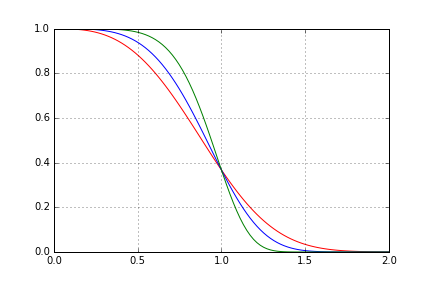
\includegraphics{images/interesting_integrals_05_1.png}
\end{figure}

Something else is interesting: We can substitute \(x=u^2\) in the
definition of the gamma function.
\(\frac{dx}{du}=2u \rightarrow dx=2u du\) and we obtain

\[
\Gamma(n) = \int_0^\infty e^{-x} x^{n-1} dx = \int_0^\infty e^{-u^2} u^{2(n-1)} 2u du = 2 \int_0^\infty e^{-u^2} u^{2n-1} du
\]

We can simplify the integral (and complicate the expression in the gamma
function); i.e.~we have

\[
\int_0^\infty e^{-u^2} u^m du = \frac{1}{2} \Gamma \left( \frac{m+1}{2} \right)
\]

This substitution trick can also be extended to integrands of the form
\(e^{-u^n} u^m\) - the definite integrals can then be expressed in terms
of the gamma function.

We make the substitution
\(u^n = x \rightarrow u=x^{1/n} \rightarrow u^m = x^{m/n}\) and we have
\(\frac{du}{dx} = \frac{1}{n}x^{1/n - 1}\). Using this, we obtain

\[
\int_0^\infty e^{-u^n} u^m du = \int_0^\infty e^{-x} x^{m/n} \frac{1}{n} x^{1/n-1} dx = \frac{1}{n} \int_0^\infty  e^{-x} x^{m/n + 1/n - 1} dx = \frac{1}{n} \Gamma \left( \frac{m+1}{n} \right)
\]

\subsection{Beta Function}

The Beta function is defined as

\[
B(m,n) = \int_0^1 x^{m-1} (1-x)^{n-1} dx, \quad m,n > 0
\]

From above we know that we can rewrite the Gamma function

\[
\Gamma(n) = 2 \int_0^\infty e^{-u^2} u^{2n-1} du
\]

Note that the integral does not depend on the name of the integration
variable; therefore we can write

\[
\Gamma(m) \Gamma(n) = 4 \int_0^\infty e^{-x^2} x^{2n-1} dx \int_0^\infty e^{-y^2} y^{2m-1} dy = 4 \int_0^\infty \int_0^\infty e^{-(x^2+y^2} x^{2m-1} y^{2n-1} du
\]

We can express this integral in terms of polar coordinates;
\(r^2 = x^2 + y^2\) and \(dx dy = r dr d\phi\):

\[
\Gamma(m) \Gamma(n) = 4 \int_{r=0}^\infty \int_{\phi=0}^{pi/2}  e^{-r^2} (r \cos \phi)^{2m-1} (r \sin \phi)^{2n-1} r dr d\phi
\]

which we can rewrite as follows

\[
\Gamma(m) \Gamma(n) = \left[ 2 \int_{r=0}^\infty e^{-r^2} r^{2(m+n)-1} dr \right] \left[  \int_{\phi=0}^{pi/2}   (\cos \phi)^{2m-1} (\sin \phi)^{2n-1} d \phi \right]
\]

The first expression in brackets is simply \(\Gamma(m+n)\), for the
second expression we substitute \(x=\cos^2 \phi\) in the Beta function

\[
B(m,n) = \int_0^1 x^{m-1} (1-x)^{n-1} dx = -2 \int_{\pi/2}^0 (\cos \phi)^{2m-2} (\sin \phi)^{2n-2} sin\phi \cos\phi d\phi
\]

where we have used \(dx =+ -2 \sin \phi \cos \phi d \phi\) and
\(1 - x = \sin^2 \phi\). But this is exactly the second expression
above; and therefore we have

\[
\Gamma(m) \Gamma(n) = \Gamma(m+n) B(m,n)
\]

\subsubsection{Plots}

The following Figure shows the integrand for various values of m and n:
Red corresponds to \(m=2, n=2\), blue corresponds to \(m=3, n=1\), green
corresponds to \(m=1, n=3\), and black corresponds to \(m=n=3\).

\begin{figure}[H]
\centering
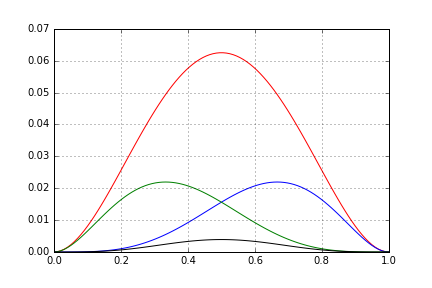
\includegraphics{images/interesting_integrals_05_2.png}

\end{figure}

The integrand is symmetric with respect to \(m,n\); therefore the Beta
function is symmetric in \(m,n\); i.e. \(B(m,n) = B(n,m)\).

The Figure below shows a contour plot of the Beta function.

\begin{figure}[H]
\centering
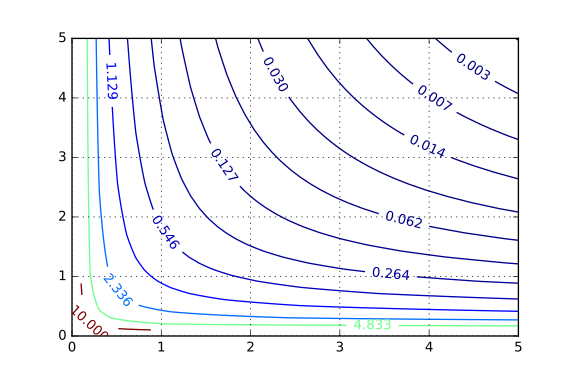
\includegraphics{images/interesting_integrals_05_3.png}
\end{figure}

\subsubsection{Properties}

The special values of \(B(m,1)\) and \(B(m,2)\) equal

\[
B(m,1) = \int_0^1 x^{m-1} (1-x)^0 dx = \left. \frac{x^m}{m} \right|_0^1 = \frac{1}{m}
\]

and

\[
B(m,2) = \int_0^1 x^{m-1} (1-x)^1 dx = \left. \frac{x^m}{m} - \frac{x^{m+1}}{m+1} \right|_0^1 = \frac{1}{m} - \frac{1}{m+1} = \frac{1}{m(m+1)}
\]

Calculating \(B(m,m)\) does not seem to be so easy; the first values are
\(B(1,1)=1, B(1,1)=1, B(2,2)=1/6, B(3,3)=1/30, B(4,4)=1/140, B(5,5)=1/630\).
I have no idea if there is a closed expression for this and what it is
(if it even exists). Neither does
\href{https://oeis.org/search?q=1\%2C6\%2C30\%2C140\%2C630\&language=german\&go=Suche}{OEIS}\ldots{}

We have \(B(m,n) = B(m,n+1) + B(m+1,n)\) by the following reasoning:

\[
B(m,n+1) + B(m+1,n) = \int_0^1 x^{m-1} (1-x)^{n} dx + \int_0^1 x^{m} (1-x)^{n-1} dx = \int_0^1 x^{m-1} (1-x)^{n-1} \left[(1-x) + x\right] dx = \int_0^1 x^{m-1} (1-x)^{n-1} dx = B(m,n)
\]

Another property is \(B(m,n) = \frac{m-1}{n} B(m-1, n+1)\) which we can
show by integration by parts (\(v = x^{m-1}, u' = (1-x)^{n-1}\)):

\[
B(m,n) = \int_0^1 x^{m-1} (1-x)^{n-1} dx = \left. \frac{1}{n} (1-x)^n x{m-1} \right|_0^1 + \int_0^1 \frac{1}{n} (1-x)^n (m-1) x^{m-2} dx
\]

The first summand becomes zero and the integral can be further
simplified to

\[
B(m,n) = \frac{m-1}{n} \int_0^1 x^{m-2} (1-x)^n dx = \frac{m-1}{n} B(m-1, n+1)
\]

There are also \(B(m+1,n)= \frac{m}{m+n}B(m,n)\) and
\(B(m,n+1)=\frac{n}{m+n}B(m,n)\) which can be proven as follows:

\[
B(m+1,n) = \frac{\Gamma(m+1)\Gamma(n)}{\Gamma(m+n+1)} = \frac{m \Gamma(m)\Gamma(n)}{\Gamma(m+n)} = \frac{m}{m+1}B(m,n)
\]

where we have used \(\Gamma(m+1) = m \Gamma(m)\). The second identity
follows analogously.

Doing this a bit more extensively, we arrive at

\[
B(m+1,n+1) = \frac{mn}{(m+n+1)(m+n)}B(m,n)
\]

With the recursion start \(B(1,1) = 1\), we can recursively calculate
the values for the Beta function.

Using the substitution \(x = y/(1+y)\) we arrive at a different
definition of the Beta function. We have \(1 - x = 1/(1+y)\) and
differentiating both sides with respect to \(y\), we obtain

\[
-\frac{dx}{dy} = -\frac{1}{(1+y)^2} \rightarrow \frac{dx}{dy} = \frac{1}{(1+y)^2}
\]

With \(y = x/(1-x)\), the limits of the integral become
\(x=0 \rightarrow y=0\) and \(x=1 \rightarrow y=\infty\) and we finally
obtain

\[
B(m,n) = \int_0^1 x^{m-1} (1-x)^{n-1} dx = \int_0^\infty \frac{y{m-1}}{(1+y){m-1}} \frac{1}{(1+y){n-1}} \frac{1}{(1+y)^2} dy = \int_0^\infty \frac{y^{m-1}}{(1+y)^{m+n}} dy
\]

Using the binomial expansion \((1-x)^n = \sum_k {n \choose k} (-x)^k\)
we arrive at

\[
B(m,n) = \int_0^1 x^{m-1} \sum_k {n-1 \choose k} (-x)^k dx = \int_0^1 \sum_k {n-1 \choose k} x^{m-1} (-x)^k dx
\]

which is - well - probably somehow useful.

\subsubsection{Applications}

The integral

\[
\int_0^{\pi/2} \sqrt{\sin x} dx
\]

can be solved by making the substitution \(u=\sin^2 x\): We have
\(du/dx = 2 \sin x \cos x\) which can be expressed (using
\(\sin x= \sqrt{u}, \cos x = \sqrt{1-u}\)) as

\[
\int_0^1 u^{1/4} \frac{du}{2\sqrt{u}\sqrt{1-u}} = \frac{1}{2} \int_0^1 u^{1/4} u^{-1/2} (1-u)^{-1/2} du = \frac{1}{2} \int_0^1 u^{-1/4} (1-u)^{-1/2} du = \frac{1}{2} B(3/3,1/2)
\]
